\chapter{計測したプログラム}
\label{cha:program}
計測に使用したプログラムは\cite{Benchmark}を参考にして自作し計測を行った。
\section{バブルソート}
数字のソートに関する性能を評価するために、バブルソートを行うプログラムを作成した。
バブルソートはソートアルゴリズムの一つで実行の速度が遅く実用的ではないが、仕組みが理解しやすいため初学者の学習によく使われる。
このアルゴリズムは、隣合う数字の大小を比べて入れ替えをすべての要素について行う。一度目の比較が終わると、数列の最大値が確定し、右端に移動した状態になる。
次に、この動作を確定した最大値をのぞいた数列で行うことを繰り返すことでソートを行う。

Python3で実装したものを図\ref{fig:b-rb}に示す。
このプログラムはテキストファイルから数列を読み取り、ソートした結果をテキストファイルに書き込む。
図\ref{fig:b-rb}の1行目で関数bsort()を定義しており、2行目から6行目でアルゴリズムを実装している。
図\ref{fig:b-rb}のそのほかの処理はテキストファイルからソートする数字を取り出す処理である。
今回作成したプログラムの計算量は O$(n^{2})$ となる。
これはソートアルゴリズムとしては遅い。例えば、クイックソートの計算量はO$(n\log{n})$とバブルソートよりも計算量が少ない。
しかし、現在のコンピューターの性能では負荷の少ないクイックソートの計算は一瞬で終了してしまうため計測が難しいと考えた。
そのため本研究では、計算量が多く、スクリプト言語の差が顕著に出ることが予想されるバブルソートを計測することにした。

\section{フィボナッチ数列}
スクリプト言語の再起呼び出しの性能を測定するために、フィボナッチ数列を算出するプログラムを作成した。
フィボナッチ数列とは「1,1,2,3,5,8,13,21,34,55,89,144」という様に数列のそれぞれの数が1つ前と2つ前の数の和になっている。
フィボナッチ数列は漸化式\ref{eq:fibonacci} と表せる。
\begin{eqnarray} \label{eq:fibonacci}
  F_{0}&=&0 \nonumber \\
  F_{1}&=&1 \\
  F_{n+1}&=&F_{n}+F_{n+1}(n≥0)\nonumber
\end{eqnarray}
この漸化式を再起処理を使って再現し実装する。

Python3で実装したものを図\ref{fig:f-py}に示す。
図\ref{fig:f-py}の3行目に定義したfib()関数を7行目で再起呼び出しを行っている。
fib()の引数が0か1になるまで引数を1ずつ減らしながらfib()を呼び出し続ける。
再起呼び出しを使ったプログラムはforなどのループ処理に比べて、
関数呼び出し時の負担が何度も存在するため実行時間が増加する傾向にある。
同様に、今回のプログラムは導出する数が1大きくなるごとに再起呼び出しの回数が指数関数的に増加する。
今回作成したプログラムの計算量は O$((\frac{1 +\sqrt{5}}{2})^{n-1})$ となる。
このような時間のかかる漸化式を使った実装は避けられており実用的でない。
一般的には言語の機能の一つであるメモ化などを使って実装することが多い。
しかし、本研究では再起呼び出しに関する処理能力を計測することを目的としていたため、効率の悪い漸化式での実装を行った。

\section{円周率の算出}
スクリプト言語の計算能力を測定するために、円周率を求めるプログラムを作成した。
円周率を求めるためにライプニッツ級数を使用した。
ライプニッツ級数は次の級数\ref{eq:leibniz}と表せる。
\begin{eqnarray} \label{eq:leibniz}
\sum_{n=0}^{\infty}\frac{(-1)^n}{2n+1}=\frac{\pi}{4}
\end{eqnarray}
また、この式は式\ref{eq:leibniz2}と表せる。
\begin{eqnarray} \label{eq:leibniz2}
1-\frac{1}{3}+\frac{1}{5}-\frac{1}{7}+\cdots=\frac{\pi}{4}
\end{eqnarray}
級数の実行回数を増やすと円周率の精度が上がる。
10億回程度実行すると円周率が10桁まで正しく算出される。
円周率の計算方法の中では収束が遅く効率は悪いが、
現在のコンピューターでその他の方法を使うと非常に早く収束してしまい測定が難しい。
よって、ライプニッツ級数はプログラミング言語の性能を測るのに適していると考えた。

Python3で実装したものを図\ref{fig:p-py}に示す。
図\ref{fig:p-py}では6行目から9行目を使い式\ref{eq:leibniz}の左辺を再現している。
また、10行目で左辺を4倍することでπを求めている。
またPHPで実装したものを図\ref{fig:p-php}に示す。
2行目から11行目で級数の実装をしており、その他の部分は導出した解をテキストファイルに書き込み処理である。
この二つを比べると級数の実装方法にはほぼ差異がないことがわかる。
残りの2つのスクリプト言語での実装に関しても、同じような計算量になるように注意して記述を行った。
このプログラムの計算量はO(n)となり、実行回数に比例する。

\section{正規表現}
スクリプト言語の正規表現に関する処理能力を測定するためにURLを判別するプログラムを作成した。
任意の行数のurlが混ざったテキストファイルを開き、そのデータから正規表現を使ってURLを取り出し出力する。
URLの判別には正規表現を使う。行の数を増やしていき、実行の速度を測る。

Python3で実装したものを図\ref{fig:s-py}に示す。
図\ref{fig:s-py}では正規表現を扱うライブラリ"re"をインポートして関数re.findallを使用していることがわかる。
また、PHPで書かれたプログラム図\ref{fig:s-php}ではpreg-match関数が使われている。
これらの関数は結果としては同じふるまいをする関数だが、言語ごとに実行速度が異なる結果になることが予想できた。

\begin{lstlisting}[label={prg:gst}, caption={GStreamer コマンドライン}, basicstyle=\ttfamily\footnotesize, frame=single]
gst-launch-1.0 -v rtmpsrc location=rtmp://localhost/live/live \
! flvdemux ! h264parse ! decodebin ! videoscale add-borders=true \
! video/x-raw,width=888,height=480 \
! x264enc bitrate=900 speed-preset=1 tune=zerolatency \
! rtph264pay config-interval=-1 pt={pt} \
! udpsink host=127.0.0.1 port={port}
\end{lstlisting}

\begin{figure}[tb]
    \centering
    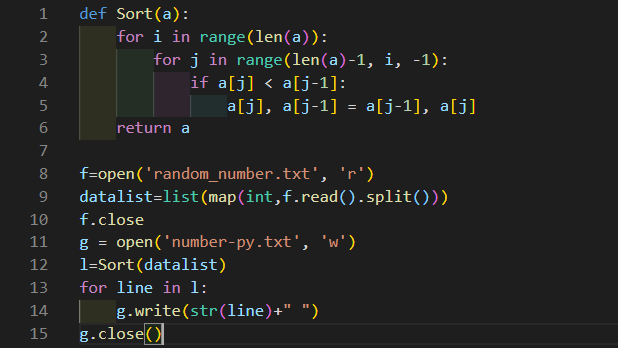
\includegraphics[width=13.5cm,keepaspectratio]{figure/b-rb.PNG}
    \caption{Python3 バブルソート}
    \label{fig:b-rb}
\end{figure}

\begin{figure}[tb]
    \centering
    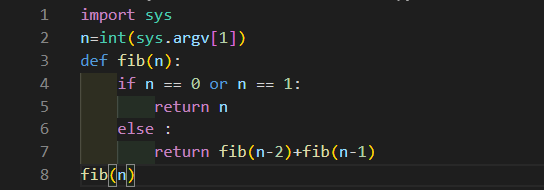
\includegraphics[width=13.5cm,keepaspectratio]{figure/f-py.PNG}
    \caption{Python3 フィボナッチ数列}
    \label{fig:f-py}
\end{figure}

\begin{figure}[tb]
    \centering
    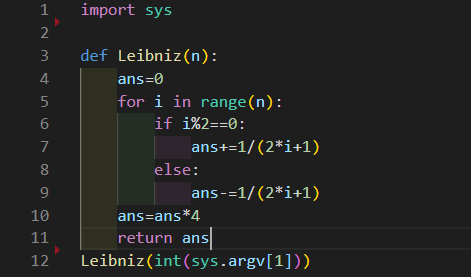
\includegraphics[width=13.5cm,keepaspectratio]{figure/p-py.PNG}
    \caption{Python3 円周率の算出}
    \label{fig:p-py}
\end{figure}

\begin{figure}[tb]
    \centering
    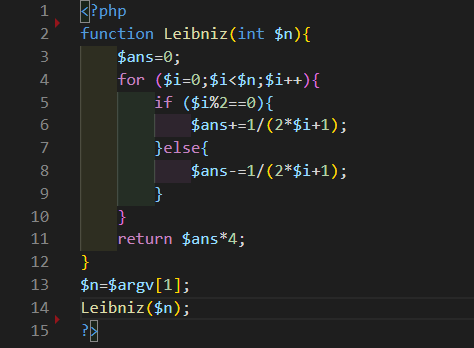
\includegraphics[width=13.5cm,keepaspectratio]{figure/p-php.PNG}
    \caption{PHP 円周率の算出}
    \label{fig:p-php}
\end{figure}

\clearpage
\begin{figure}[tb]
    \centering
        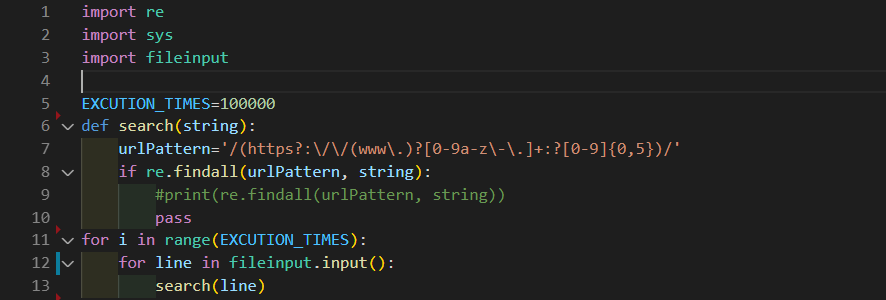
\includegraphics[width=13.5cm,keepaspectratio]{figure/s-py.PNG}
        \caption{Python3 正規表現}
        \label{fig:s-py}
\end{figure}

\begin{figure}[tb]
    \centering
        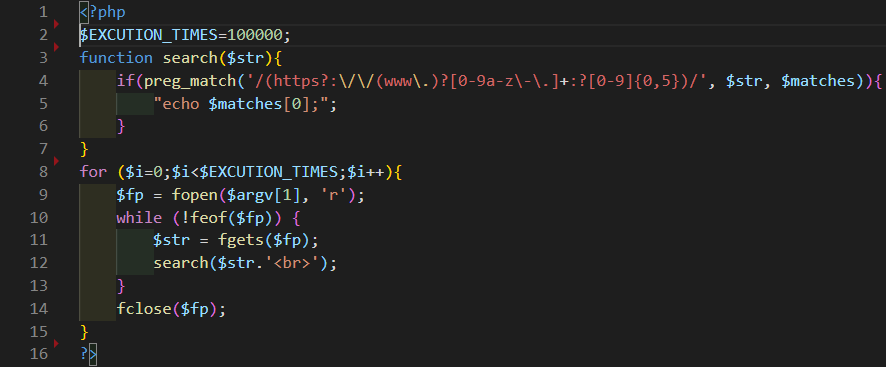
\includegraphics[width=13.5cm,keepaspectratio]{figure/s-php.PNG}
        \caption{PHP 正規表現}
        \label{fig:s-php}
\end{figure}